\documentclass[a4paper,12pt]{article}
\usepackage[czech]{babel}
\usepackage{graphicx}
\usepackage{geometry}
\geometry{a4paper, margin=1in}


% Packages
\usepackage{amsmath}
\usepackage{graphicx}
\usepackage{float}
\usepackage{longtable}
\usepackage{hyperref}
\usepackage{url}
\usepackage{setspace}
\onehalfspacing
\setlength{\parindent}{0pt}  % No paragraph indentation
\setlength{\parskip}{1em}    % Space between paragraphs

\usepackage[backend=biber,style=authoryear]{biblatex}
\addbibresource{zdroje.bib}

\begin{document}

\begin{titlepage}
    \begin{center}
        {\huge \bfseries Algoritmy počítačové kartografie}\\
        \vspace{3.5em}
        {\Large \bfseries Úloha 1} \\
        \vspace{0.5em}
        {\Large \bfseries Geometrické vyhledání bodu} \\
        \vspace{3.5em}
        {\large František Macek, Josef Zátka} \\
        \vspace{2.5em}
        
\includegraphics[width=10cm]{logo.png}\\
        \vspace{-2em}
        { \bfseries Univerzita Karlova}\\
        \vspace{0.33em}
        { \bfseries Přírodovědecká fakulta}\\
        \vspace{0.33em}
        { \bfseries Katedra aplikované geoinformatiky a kartografie}\\
        \vspace{10em}
        {\large Praha, 2025}
    \end{center}
\end{titlepage}

\section{Zadání}

Vstup: Souvislá polygonová mapa $n$ polygonů $\{P_1, ..., P_n\}$, analyzovaný bod $q$.

Výstup: $P_i$,  $q \in P_i$. 
Nad polygonovou mapou implementujete \textit{Ray Crossing Algorithm} pro geometrické vyhledání incidujícího polygonu obsahujícího zadaný bod $q$.

Nalezený polygon graficky zvýrazněte vhodným způsobem (např. vyplněním, šrafováním, blikáním). Grafické rozhraní vytvořte s využitím frameworku \textit{QT}. Pro generování nekonvexních polygonů můžete navrhnout vlastní algoritmus či použít existující geografická data (např. mapa evropských států).

Polygony budou načítány z textového souboru ve Vámi zvoleném formátu. Pro datovou reprezentaci jednotlivých polygonů použijte špagetový model.

\section{Údaje o bonusových úlohách}

Byly zprácovány následující bonusové úlohy s uvedeným bodovým ohodnocením:

\begin{small}
\begin{longtable}{|p{12cm}|c|}
    \hline
    \textbf{Krok} & \textbf{Hodnocení} \\
    \hline
    \endfirsthead
    
    \hline
    \textbf{Krok} & \textbf{Hodnocení} \\
    \hline
    \endhead

    Detekce polohy bodu rozlišující stavy uvnitř, vně polygonu. & 10b \\
    \hline
    \textit{Analýza polohy bodu (uvnitř/vně) metodou Winding Number Algorithm.} & +10b \\
    \hline
    Ošetření singulárního případu u Winding Number Algorithm: bod leží na hraně polygonu. & +5b \\
    \hline
    Ošetření singulárního případu u Ray Crossing Algorithm: bod leží na hraně polygonu. & +5b \\
    \hline
    Ošetření singulárního případu u obou algoritmů: bod je totožný s vrcholem jednoho či více polygonů. & +2b \\
    \hline
    Zvýraznění úsech polygonů pro oba výše uvedené singulární případy. & +3b \\
    \hline
    Rychlé vyhledání potenciálních polygonů (bod uvnitř min-max boxu). & +10b \\
    \hline
    Načtení vstupních dat ze *.shp. & +10b \\
    \hline
    \textbf{Celkem splněno:} & \textbf{55b} \\
    \hline
\end{longtable}
\end{small}

\section{Úvod, popis a rozbor problematiky}

Jedním z často řešených problémů v oblasti počítačové grafiky a digitální kartografie je určování vztahu mezi polohou daného bodu a polygonem. Tento úkol, známý jako problém bodu v polygonu (Point Location Problem), slouží k určení, zda se bod nachází uvnitř, vně nebo na hranici daného polygonu \parencite{bayer_prednaska}.

Existují dvě hlavní techniky řešení problému bodu v polygonu \parencite{bayer_prednaska}:

\begin{enumerate}
    \item \textbf{Převod problému na vztah bodu a mnohoúhelníku} – Opakovaně určujeme polohu bodu vzhledem k polygonu. Tato metoda je snadno implementovatelná, ale pomalejší.
    \item \textbf{Planární dělení roviny} – Rovina je rozdělena na pásy nebo lichoběžníky, čímž vzniká trapezoidální mapa. Tato technika je výrazně rychlejší, ale složitější na implementaci, vyžaduje speciální datové struktury (např. binární stromy).
\end{enumerate}

Řešení problému se dále liší v závislosti na tom, zda do problému vstupují pouze konvexní polygonu, nebo také polygony nekonvexní. Pro konvexní polygony (ty mají vnitřní úly o maximální velikosti 180°) je řešení výpočetně jednodušší. V geoinformatice a kartografii se ovšem běžně setkáváme s polygony nekonvexními, a tak je i v této úloze problém řešen pro nekonvexní polygony.

Mezi základí algoritmy pro řešení problému bodu v nekonvexním polygonu jsou řazeny Ray Crossing Algorithm a Winding Number Algorithm. Ty byly v této úloze implementovány a v dalších kapitolách jsou podrobněji popsány.



\section{Ray Crossing Algorithm}
\subsection{Popis algoritmu}

Základním principem \textit{Ray Crossing Algorithm} je vysílání "paprsku" ze zvoleného bodu \textit{q} do jednoho směru. Tento paprsek tvoří polopřímku, která \textit{k} krát protne obálku polygonu \textit{P}. Na základě počtu průsečíku lze určit, zda bod \textit{q} leží uvnitř či vně polygonu \textit{P} dle pravidla

\[
k\%2 =
\begin{cases} 
    1, & q \in P, \\
    0, & q \notin P.
\end{cases}
\]

Tedy pokud je počet průsečíků sudý, lze říci, že bod leží vně polygonu. Je-li počet průsečíků lichý, bod leží uvnitř polygonu. Obě varianty ilustruje obrázek 1.

\begin{figure}[H]
    \centering
    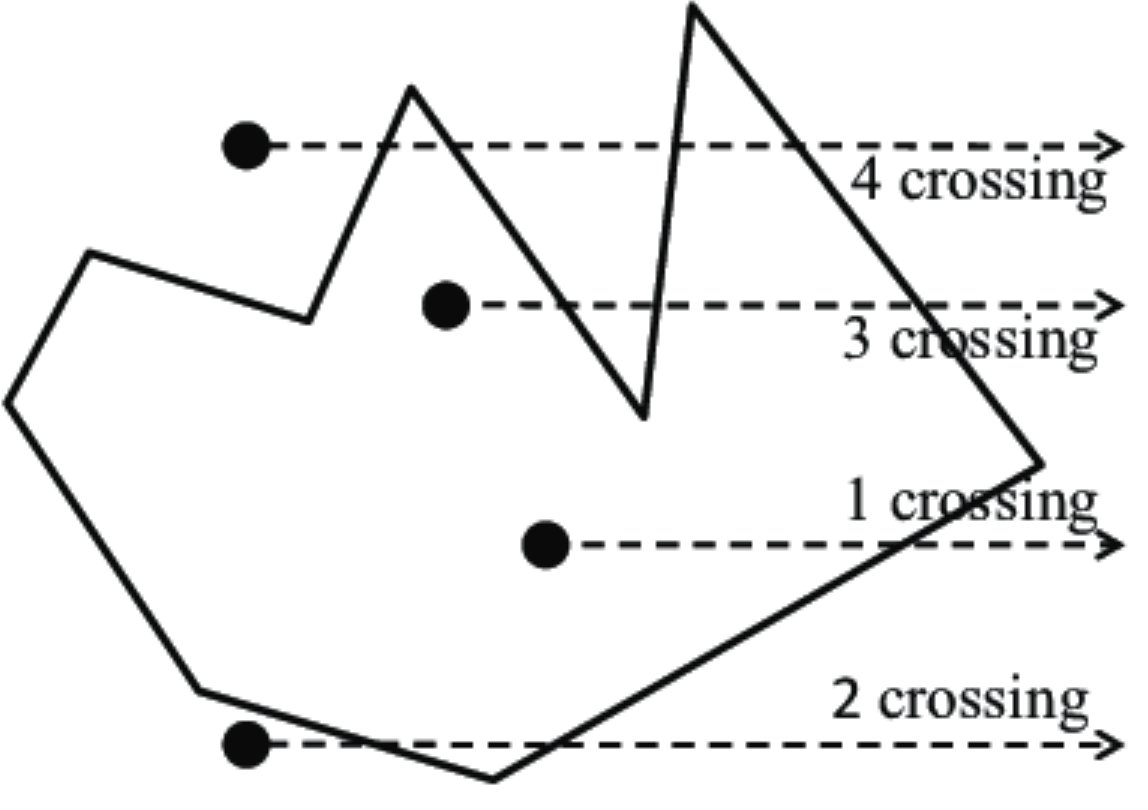
\includegraphics[width=0.4\linewidth]{ray_cross_1.PNG}
    \caption{Základní princip Ray Crossing Algorithm \parencite{obr1}}
    \label{fig:enter-label}
\end{figure}

V praxi je jako paprsek volena polopřímka rovnoběžná s osou x, která míří od bodu \textit{q} v kladném směru osy x \parencite{geeks}.

V algoritmu je polygon reprezentován jako uspořádaná posloupnost bodů, dvojice po sobě jdoucích bodů tedy tvoří hrany takového polygonu. Abychom zjistili, zda paprsek procházející bodem \textit{q} protíná polygon, musíme pro každou hranu polygonu prověřit, zda protíná vytyčenou polopřímku.

Každá hrana je určena dvěma sousedními vrcholy polygonu
\[
p_i = (x_i, y_i), \quad p_{i+1} = (x_{i+1}, y_{i+1}).
\]

Pro každý úsek \([p_i, p_{i+1}]\) jsou vypočítány relativní souřadnice vůči bodu \textit{q} jako

\[
x'_i = x_i - x_q, \quad y'_i = y_i - y_q
\]
\[
x'_{i+1} = x_{i+1} - x_q, \quad y'_{i+1} = y_{i+1} - y_q
\]

Tyto transformované souřadnice umožňují pracovat s bodem \textit{q} jako novým počátkem souřadnicového systému. Díky tomu lze snadněji testovat, zda hrana protíná vodorovnou polopřímku v kladném směru osy x.

Aby hrana protnula paprsek, musí splňovat podmínku

\[
(y'_i > 0 \land y'_{i+1} \leq 0) \quad \text{nebo} \quad (y'_i \leq 0 \land y'_{i+1} > 0)
\]

Tato podmínka zajišťuje, že úsečka kříží osu x (tedy paprsek).

Pokud podmínka platí, pak je vypočtena souřadnice průsečíku hrany s osou x:

\[
x_m = \frac{x'_{i+1} y'_i - x'_i y'_{i+1}}{y'_{i+1} - y'_i}
\]

Pokud je \( x_m > 0 \), znamená to, že průsečík \textbf{leží napravo od bodu \( q \)}, a tedy \textbf{započítáme ho jako průsečík s paprskem}.

Po vyhodnocení každé hrany lze dle pravidla o sudosti celkového počtu průsečíků (viz výše) rozhodnout o tom, zda bod leží uvnitř nebo vně polygonu.



\subsection{Singulární případy}
\subsubsection{Bod na hraně polygonu}
Leží-li bod na hraně polygonu či na prodloužení vodorovné hrany, vyjde \[
x_m = 0,
\]
tehdy proběhne (v naší implementaci) ověření, zda bod leží uvnitř minmax boxu tvořeného ověřovanou hranou. Pokud ano, bod leží na této hraně. Pokud nikoliv, bod leží vně polygonu.

\subsubsection{Bod leží ve vrcholu polygonu}
Další singularitou je situace, při které bod je vrcholem polygonu. V takovém případě by byl započítán jako průsečík každé hrany vedoucí z vrcholu. Tato singularita je řešena před samotným během programu tím, že je ověřeno zda bod není totožný s jedním z vrcholů polygonu.




\section{Winding Number Algorithm}
\subsection{Popis algoritmu}
\textit{Winding Number Algorithm} je druhou implementovanou technikou pro určení, zda bod \textit{q}  leží uvnitř nebo vně polygonu \textit{P}. Tento algoritmus vyhodnocuje, jak moc se polygon "obtáčí" kolem daného bodu pomocí výpočtu součtu úhlových změn mezi sousedními vrcholy polygonu vůči bodu \textit{q}. 

Princip algoritmu spočívá ve výpočtu celkového úhlového přírůstku \textit{Omega}, který vzniká postupným měřením úhlů mezi sousedními hranami polygonu a testovaným bodem. Po sečtení těchto úhlů platí následující pravidlo:

\[
\left| \Omega \right| \approx 2\pi \Rightarrow q \in P
\]

\[
\left| \Omega \right| < 2\pi \Rightarrow q \notin P
\]

Tedy pokud je absolutní hodnota součtu úhlů přibližně \( 2\pi \), bod se nachází uvnitř polygonu. Pokud je menší, bod leží vně. Princip je ilustrován na obrázku 2.

\begin{figure}[H]
    \centering
    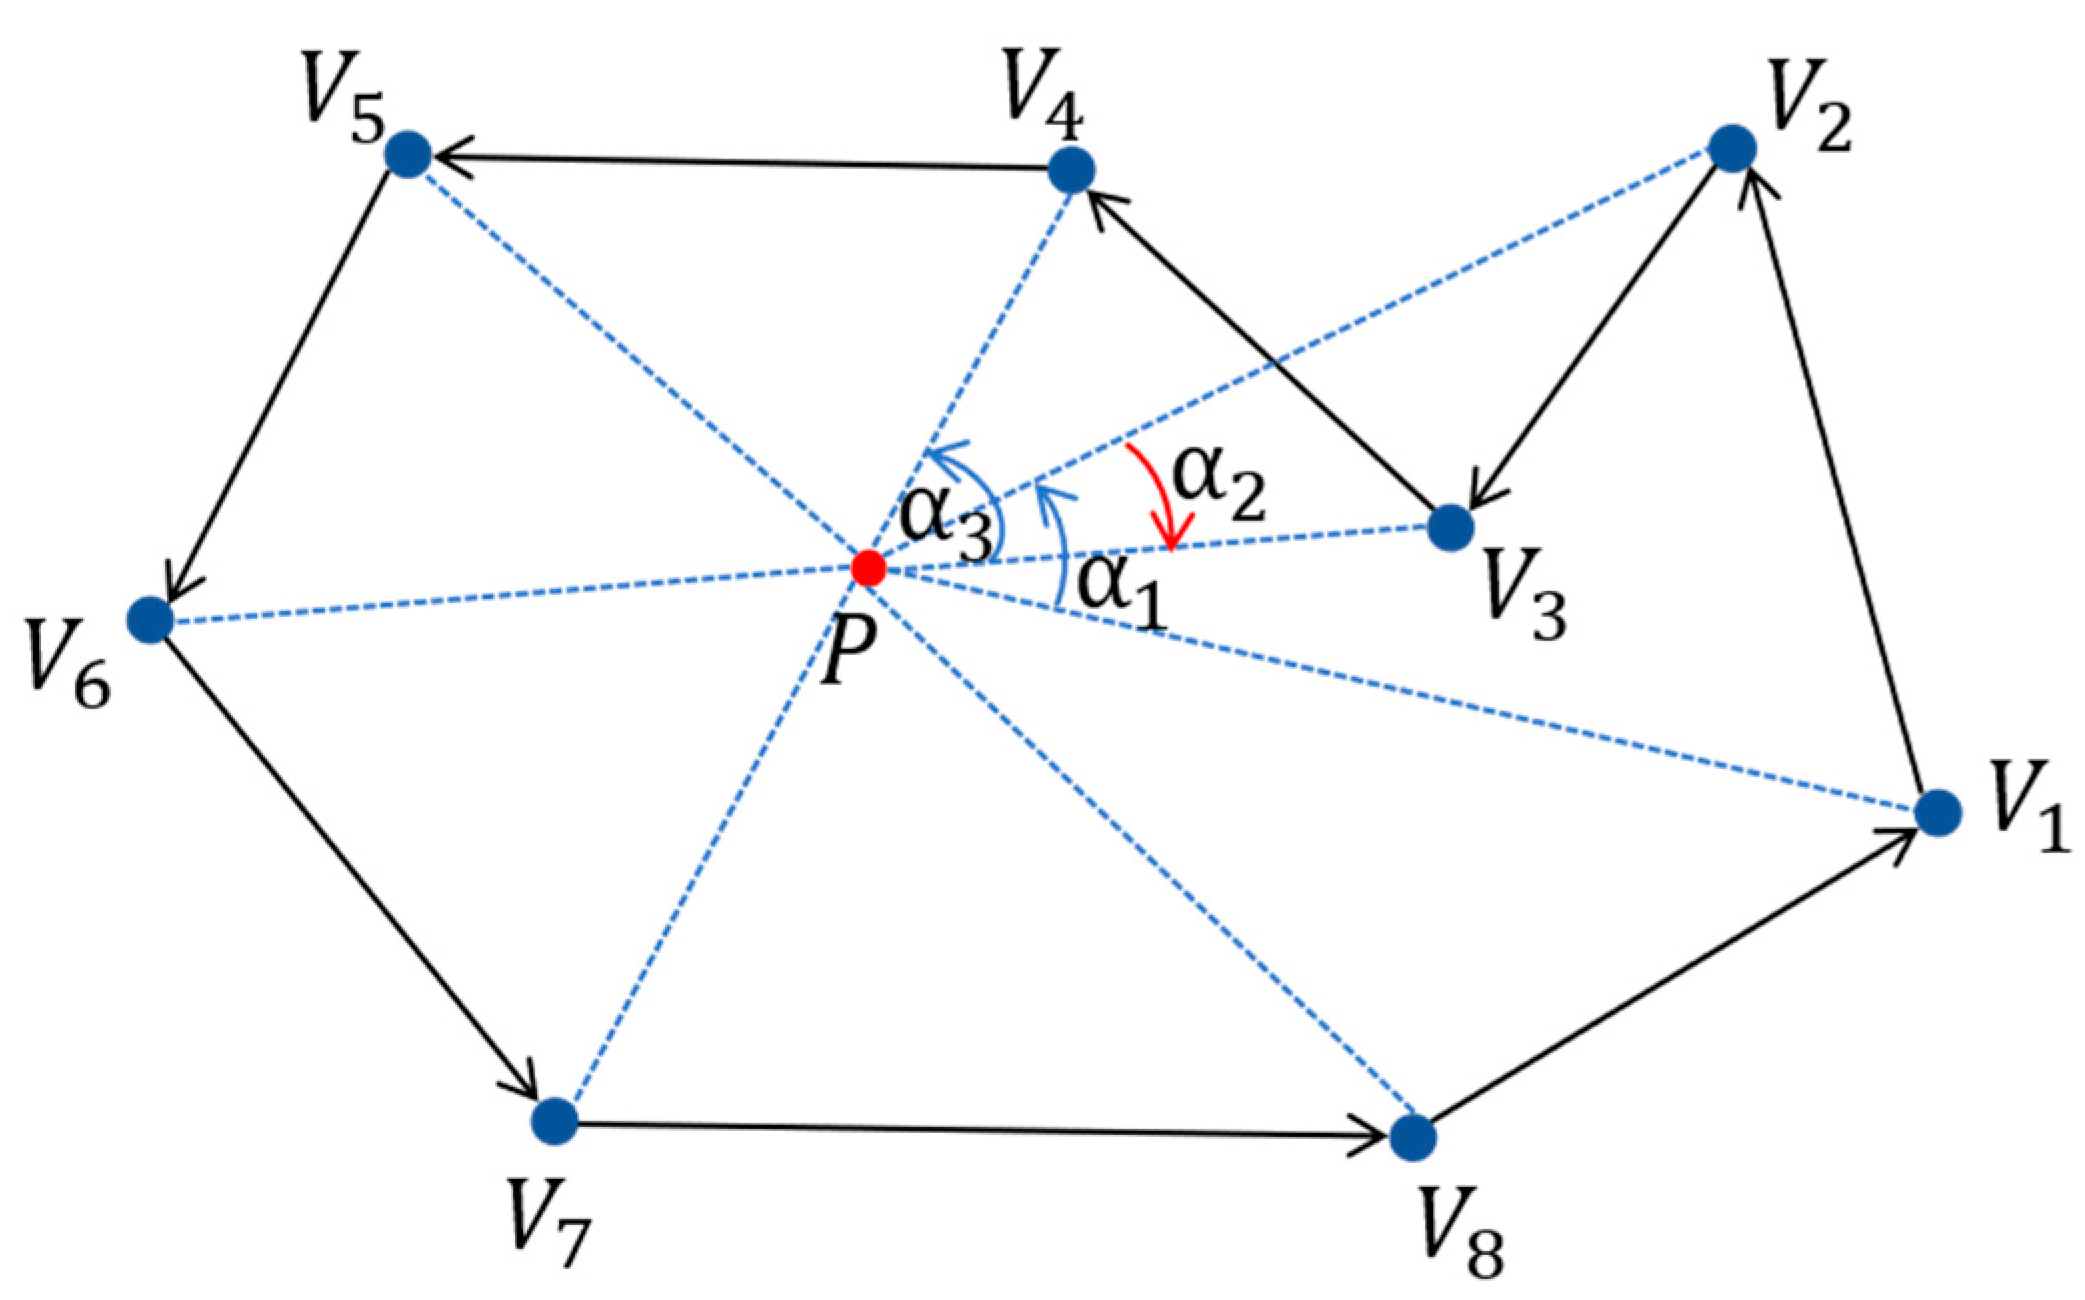
\includegraphics[width=0.6\linewidth]{winding.png}
    \caption{Základní princip Winding Number Algorithm \parencite{obr2}}
    \label{fig:winding_number}
\end{figure}


Polygon je opět reprezentován jako uspořádaná posloupnost bodů, kde dvojice po sobě jdoucích bodů tvoří hrany polygonu:

\[
p_i = (x_i, y_i), \quad p_{i+1} = (x_{i+1}, y_{i+1}).
\]

Pro každý úsek \([p_i, p_{i+1}]\) jsou nejprve vypočteny vektory z bodu \textit{q} k oběma vrcholům hrany:

\[
\mathbf{v}_1 = (x_i - x_q, y_i - y_q), \quad \mathbf{v}_2 = (x_{i+1} - x_q, y_{i+1} - y_q).
\]

Následně je spočítán skalární součin těchto dvou vektorů:

\[
\mathbf{v}_1 \cdot \mathbf{v}_2 = (x_i - x_q)(x_{i+1} - x_q) + (y_i - y_q)(y_{i+1} - y_q).
\]

Velikosti vektorů jsou dány vztahem:

\[
\|\mathbf{v}_1\| = \sqrt{(x_i - x_q)^2 + (y_i - y_q)^2}, \quad \|\mathbf{v}_2\| = \sqrt{(x_{i+1} - x_q)^2 + (y_{i+1} - y_q)^2}.
\]

Úhel \( \theta_i \) mezi vektory je pak získán pomocí vztahu:

\[
\cos \theta_i = \frac{\mathbf{v}_1 \cdot \mathbf{v}_2}{\|\mathbf{v}_1\| \|\mathbf{v}_2\|}
\]

\[
\theta_i = \arccos \left( \frac{\mathbf{v}_1 \cdot \mathbf{v}_2}{\|\mathbf{v}_1\| \|\mathbf{v}_2\|} \right).
\]


Pro správné započítání úhlu je třeba určit, zda bod \textit{q} leží na levé nebo pravé straně hrany \( [p_i, p_{i+1}] \). Toho lze dosáhnout pomocí determinantového testu (označovaného v anglické terminologii jako \textit{cross product}):

\[
D = (x_{i+1} - x_i)(y_q - y_i) - (y_{i+1} - y_i)(x_q - x_i).
\]

Pokud \( D > 0 \), bod \( q \) leží \textbf{vlevo} od hrany a úhel \( \theta_i \) je \textbf{přičten} k \( \Omega \).

Pokud \( D \leq 0 \), bod \( q \) leží \textbf{vpravo} od hrany a úhel \( \theta_i \) je \textbf{odečten} od \( \Omega \).


\textbf{Po spočtení celkového součtu úhlových přírůstků \( \Omega \) se bod klasifikuje podle pravidla:}

\[
\left| \Omega - 2\pi \right| < \varepsilon \Rightarrow q \in P
\]
\[
\left| \Omega - 2\pi \right| \geq \varepsilon \Rightarrow q \notin P,
\]

kde \( \varepsilon \) představuje zvolenou toleranci pro zaokrouhlovací chyby.

\subsection{Singulární případy}
\subsubsection{Bod na hraně polygonu}
Leží-li bod na hraně polygonu či na prodloužení vodorovné hrany, vyjde cross product (determinantový test) = 0. Tehdy je opět, stejně jako v případě Ray Crossing algoritmu testováno, zda bod leží uvnitř minmax boxu ověřované hrany
tehdy proběhne (v naší implementaci) ověření, zda bod leží uvnitř minmax boxu tvořeného ověřovanou hranou. Pokud ano, bod leží na této hraně. Pokud nikoliv, bod leží vně polygonu.

\subsubsection{Bod leží ve vrcholu polygonu}
Další singularitou je opět situace, při které je ověřovaný bod vrcholem polygonu. V takovém případě by byl započítán jako průsečík každé hrany vedoucí z vrcholu. Tato singularita je řešena před samotným během programu tím, že je ověřeno zda bod není totožný s jedním z vrcholů polygonu.

\section{Vlastní implementace}
Součástí zadání bylo nejen implementovat algoritmy pro analýzu polohy bodu v prostoru, ale také navrhnout intuitivní a uživatelsky přívětivé rozhraní ve frameworku Qt. Toto rozhraní umožňuje snadnou demonstraci funkčnosti obou zmíněných algoritmů nad vybranou vrstvou polygonů, čímž uživateli poskytuje přehledný a interaktivní způsob vizualizace výsledků.

\subsection{Vstupní a výstupní data}
Aplikace umožňuje importovat polygony ze souboru formátu *.shp. Pro správné vykreslování polygonů v okně aplikace je předpokladem, že geometrie je v shapefilu uložena v souřadnicovém systému WebMercator (EPSG:3857). U něj s rostoucí zeměpisnou délkou roste hodnota souřadnice X (směrem doprava) a s klesající zeměpisnou šířkou roste hodnota soouřadnice Y (ve směru dolů). Tato vlastnost umožňuje neinvertovat souřadnici Y a rovnou ji použít na vykreslení v knihovně Qt, protože v ní je počátkem souřadnic (0,0) levý horní bod vykreslovací plochy.

Výstupem aplikace je podbarvení polygonu uvnitř kterého leží zvolený bod (obrázek 3).

\begin{figure}[H]
    \centering
    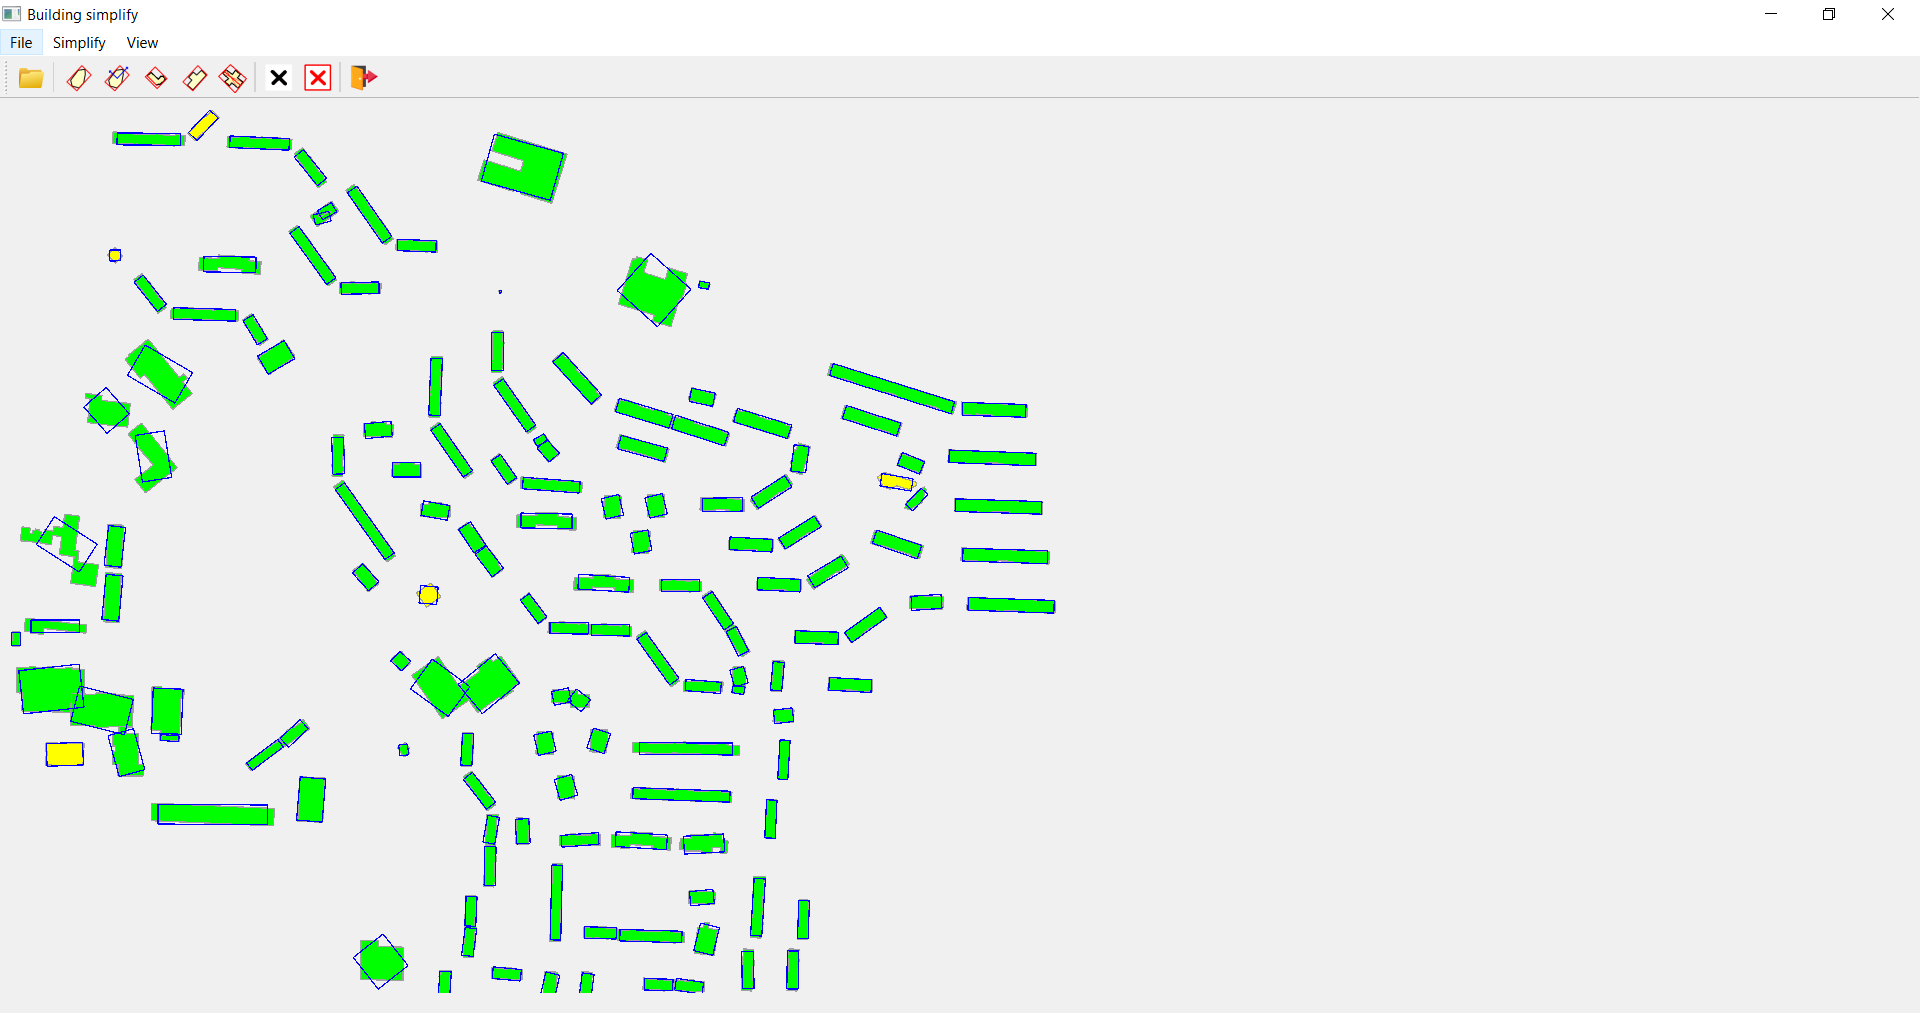
\includegraphics[width=1\linewidth]{app1.png}
    \caption{Podbaarvení polygonu uvnitř kterého leží vybraný bod}
    \label{fig:winding_number}
\end{figure}

\subsection{Aplikace}
Aplikace byla vytvořena prostřednictvím knihoven Qt v programovacím jazyce Python. 
Uživatel může otevřít soubor formátu shapefile z vlastního adresáře. Následně lze v aplikaci levým tlačítkem myši zvolit bod pro analýzu jeho polohy vůči nahraným polygonům. Volby načtení souboru, analýzy jeho polohy metodou Ray Crossing a Winding Number a další operace lze spustit pomocí ikon umístěných v horní části okna aplikace (obrázek 4). Nalezený polygon, uvnitř kterého leží zvolený bod je zeleně podbarven. 

\begin{figure}[H]
    \centering
    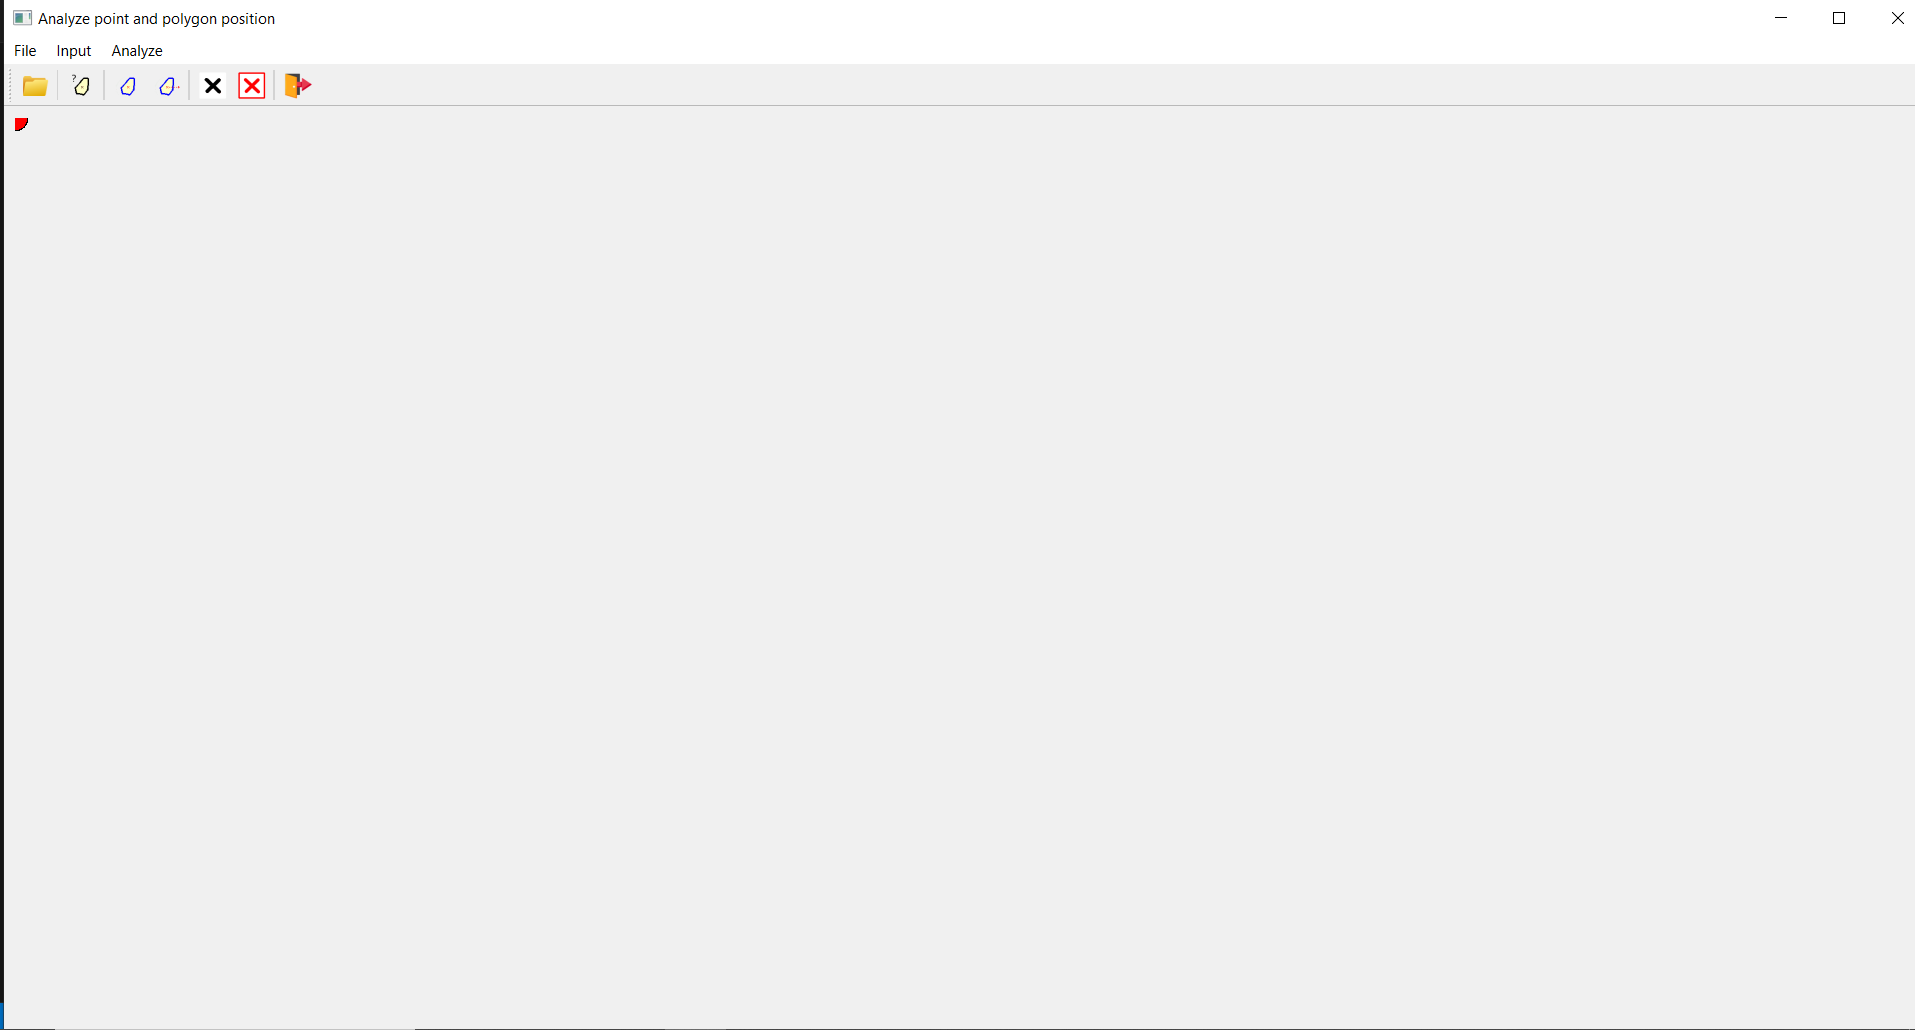
\includegraphics[width=1\linewidth]{okno.PNG}
    \caption{Okno aplikace}
    \label{fig:enter-label}
\end{figure}

Uživatel může také nahraná data vymazat ikonou červeného křížku a ukončit běh celého programu k tomu určenou ikonou.

\section{Třídy a metody tříd}
Pro zdárný běh celé aplikace jsou nezbytné soubory \texttt{MainForm.py}, \texttt{draw.py}, \texttt{algorithms.py} a \texttt{read\_shp.py}.

\subsection{Třída MainForm}
Třída zajišťuje vykreslení okna aplikace, včetně všech ikon a tlačítek. Také zajišťuje jejich propojení s metodami, které vyvolávají další akce.
Metody třídy MainForm a jejich funkce jsou následující:
\begin{itemize}
    \item \textbf{setupUi a retranslateUi} – Nastavují grafické uživatelské rozhraní aplikace, včetně rozložení, menu, toolbaru a jejich propojení s funkcemi. 
    \item \textbf{analyzeRay} – Určuje, zda bod leží uvnitř polygonu pomocí Ray-Crossing algoritmu volaného ze třídy Algorithms.
    \item \textbf{inside_bounding} – Analyzuje, zda bod leží uvnitř minmax boxu tvořeného dvěma jinými body.
    \item \textbf{analyzeWinding} – Testuje polohu bodu vůči polygonům pomocí Winding Number algoritmu volaného ze třídy Algorithms.
    \item \textbf{switchClick} – Přepíná vstup mezi bodem a polygonem.
    \item \textbf{openFileDialog} – Otevírá dialogové okno pro výběr souboru \texttt{.shp} a načítá data do vykreslovacího okna.
    \item \textbf{pointInside} – Zobrazí dialogové okno s informací, že bod je uvnitř polygonu, a zvýrazní ho.
    \item \textbf{pointOutside} – Zobrazí dialogové okno s informací, že bod je mimo polygon.
    \item \textbf{pointEdge} – Zobrazí dialogové okno s informací, že bod se nachází na hraně polygonu, a zvýrazní odpovídající polygon/y ve vykreslovacím okně.
    \item \textbf{pointVertex} – Zobrazí dialogové okno s informací, že bod se shoduje s vrcholem jednoho nebo více polygonů, a vizuálně je zvýrazní.
\end{itemize}

\subsection{Třída Draw}
Třída zajišťuje vykreslování bodů a polygonů v aplikaci a umožňuje interakci uživatele s grafickou plochou prostřednictvím stlačení tlačítka myši.
Metody třídy Draw a jejich funkce jsou následující:
\begin{itemize}
    \item \textbf{mousePressEvent} – Zaznamenává kliknutí myší, ukládá souřadnice bodu nebo přidává vrcholy k polygonu.
    \item \textbf{paintEvent} – Zajišťuje vykreslení bodů a polygonů na plátno včetně zvýraznění označeného polygonu.
    \item \textbf{paintInputEvent} – Aktualizuje seznam vykreslovaných polygonů po nahrání vstupního souboru formátu .shp.
    \item \textbf{switchInput} – Přepíná mezi režimem zadávání bodu a režimem přidávání vrcholů do polygonu.
    \item \textbf{getQ} – Vrací souřadnice označeného bodu.
    \item \textbf{getPol} – Vrací aktuální polygon.
    \item \textbf{getPolygons} – Vrací seznam všech polygonů.
    \item \textbf{highlightPolygon} – Zvýrazňuje vybraný polygon a zajišťuje překleslení plátna.
    \item \textbf{unhighlightPolygon} – Odbarví zvýrazněné polygony.
    \item \textbf{clearData} – Odstraňuje všechna data z vykreslovací plochy.
\end{itemize}

\subsection{Třída Algorithms}
Třída obsahuje algoritmy pro analýzu polohy bodu vzhledem k polygonu a výběr potenciálně relevantních polygonů.
Metody třídy Algorithms a jejich funkce jsou následující:
\begin{itemize}
    \item \textbf{ray\_crossing} – Určuje, zda bod leží uvnitř polygonu pomocí Ray-Crossing algoritmu na základě počtu průsečíků s hranicemi polygonu.
    \item \textbf{winding\_number} – Testuje polohu bodu vůči polygonu pomocí Winding Number algoritmu na základě součtu úhlů.
    \item \textbf{minmaxbox} – Vytváří ohraničující obdélník (min-max box) pro daný polygon pomocí minimálních a maximálních souřadnic jeho vrcholů.
    \item \textbf{point\_inside\_minmaxbox} – Určuje, zda bod leží uvnitř ohraničujícího obdélníku polygonu, což slouží k předběžné eliminaci nerelevantních polygonů.
    \item \textbf{select\_suspicious\_polygons} – Vyhledává a vrací seznam polygonů, jejichž minmax box obsahuje zadaný bod.
    \item \textbf{point\_vertex} – Vrací informaci o tom, zda je analyzovaný bod shodný s některým z vrcholů polygonu.
\end{itemize}

\subsection{Soubor read\_shapefiles.py}
Soubor obsahuje jedinou funkci load\_shapefile, která načítá geometrie polygonů ze souboru ve formátu \texttt{.shp} pomocí knihovny GeoPandas a následně upravuje jejich souřadnice pro vykreslení v aplikaci. Nejprve se soubor načte a získají se jeho minimální a maximální souřadnice, které určují rozsah dat. Poté se vypočítá měřítko pro přizpůsobení souřadnic velikosti okna, přičemž se zachovává poměr stran. Funkce následně prochází jednotlivé polygony, převádí jejich vrcholy na odpovídající souřadnice v okně a ukládá je jako objekty \texttt{QPolygonF}. Tímto způsobem se zajistí, že načtené polygony budou správně zobrazeny v aplikaci. Na závěr funkce vrací seznam těchto polygonů ve formátu \texttt{QPolygonF}, které lze použít pro vykreslení.


\section{Závěr}
Prostřednictvím funkční aplikace byly implementovány algoritmy Ray Crossing a Winding Number pro určení polohy bodu a polygonu. Součástí řešení je i ošetření singulárních případů, kdy bod leží na hraně polygonu či v jednom z jeho vrcholů.
Program v současné verzi nedokáže zpracovávat polygony s dírami, v této oblasti se nabízí prostor pro budoucí vylepšení. Také možnost importu vstupních polygonů je omezena pouze na soubory formátu shapefile. Vylepšením předkládaného programu by mohla být možnost importovat data  také z jiných geoprostorových formátů (např. GeoJSON). Současná verze validně vykresluje pouze shapefily se souřadnicovým systémem WebMercator, podpora jiných souřadnicových systémů.
Vhodným vylepšením by také byla možnost posouvání a přibližování//oddalování plochy na které jsou vykresleny polygony.
Vytvořená aplikace je uživatelům dostupná na adrese \href{https://github.com/Omactek/task_1/tree/main}.

\printbibliography[title={Zdroje}]



\end{document}